\documentclass[11pt]{article}
% Guía «Cómo cantar un tema» de Víctor Gutiérrez Marcos, con el estilo del temario
% (tcee.sty). Se compila con oposicion/temario/latex en TEXINPUTS:
%   TEXINPUTS=../../temario/latex//: pdflatex como-cantar-un-tema.tex  (dos pasadas)
% Las cifras de los patrones salen de los 90 temas revisados del tercer
% ejercicio (fuentes/*/*.tex, 20/11/2026).
\usepackage{tcee}
\usetikzlibrary{arrows.meta,positioning,calc,shapes.symbols,shapes.misc,fit,backgrounds,matrix}
\tcetema[Cómo cantar un tema]{Guía}{Cómo cantar un tema}
\tcefecha{20/11/2026}
\tceeguia
\hypersetup{pdftitle={Cómo cantar un tema},pdfsubject={Guía para cantar un tema de la oposición a TCEE: método y patrones del temario}}

% --- Estilos de las infografías -------------------------------------------------
\tikzset{
  inf/.style={font=\footnotesize,line cap=round,line join=round,>={Stealth[length=2.2mm]}},
  paso/.style={rectangle,rounded corners=2pt,fill=tceemorado,text=white,font=\small\bfseries,
    text width=2.75cm,align=center,inner sep=4pt,minimum height=1.05cm},
  pasoclaro/.style={paso,fill=tceemorado!55},
  pasodorado/.style={paso,fill=tceedorado},
  que/.style={rectangle,rounded corners=2pt,fill=tceemoradopalido,draw=tceemorado!35,
    text width=4.3cm,align=left,inner sep=4pt,font=\footnotesize},
  ejemplo/.style={rectangle,rounded corners=2pt,fill=tceesalvia,draw=tceesalviaoscuro,
    text width=7.35cm,align=left,inner sep=4pt,font=\footnotesize\itshape},
  pizarra/.style={rectangle,rounded corners=1pt,fill=white,draw=tceegris,line width=0.6pt,
    text width=4.3cm,align=center,inner sep=4pt,font=\footnotesize},
  cabecera/.style={font=\footnotesize\bfseries\color{tceemorado},align=center},
  nexo/.style={rectangle,rounded corners=2pt,fill=tceesalvia,draw=tceesalviaoscuro,
    text width=11.6cm,align=left,inner sep=3pt,font=\footnotesize\itshape},
  flechamorada/.style={->,thick,tceemorado},
  pregunta/.style={rectangle,rounded corners=6pt,draw=tceemorado,line width=0.8pt,fill=white,
    text width=4.4cm,align=center,inner sep=5pt,font=\footnotesize\bfseries},
  resultado/.style={rectangle,rounded corners=2pt,text width=9.4cm,align=left,inner sep=5pt,
    font=\footnotesize,line width=0.8pt},
  cifra/.style={rectangle,rounded corners=2pt,fill=tceemoradopalido,draw=tceemorado!40,
    text width=3.45cm,align=center,inner sep=4pt,font=\footnotesize,execute at begin node={\hyphenpenalty=10000\exhyphenpenalty=10000}},
}
% Rótulo de las infografías: en negrita y morado
\makeatletter\setlength{\@fptop}{0pt}\setlength{\@fpbot}{0pt plus 1fil}\makeatother
\renewcommand{\topfraction}{0.95}\renewcommand{\bottomfraction}{0.9}\renewcommand{\textfraction}{0.05}\renewcommand{\floatpagefraction}{0.85}
\newcommand{\rot}[1]{{\bfseries\color{tceemorado}#1}}
\newcommand{\rotb}[1]{{\bfseries\color{white}#1}}
% Tarjetas de patrones
\newcommand{\tarjeta}[3]{%
  \begin{tcolorbox}[enhanced,colback=white,colframe=#1,boxrule=0.7pt,arc=2pt,
    title={#2},fonttitle=\small\bfseries\raggedright,colbacktitle=#1,coltitle=white,
    fontupper=\footnotesize,left=5pt,right=5pt,top=3pt,bottom=3pt]#3\end{tcolorbox}}
\newcommand{\fila}[2]{\par\noindent{\bfseries\color{tceemoradooscuro}#1}\enspace #2\par\vspace{1.5pt}}

\begin{document}
\tceetitulo

\begin{notaopositor}
El temario de esta oposición es libre en todo lo que esté más allá del respeto al título de cada tema, por lo que no existe un tema único posible y, en consecuencia, estos temas no pretenden serlo.
\begin{itemize}
\item La exposición oral del tema, aunque deba ser clara y didáctica, \emph{no es una clase}: no es necesario explicar durante ella (aunque sí conocer) los modelos y la teoría con todo detalle. No pretende ser una clase magistral, sino dar los elementos y resultados fundamentales y las intuiciones económicas más poderosas.
\item El opositor es responsable de su necesaria \emph{personalización}, ya sea síntesis, simplificación, reestructuración o extensión. Esta adaptación a las circunstancias personales (conocimientos previos, forma de estudio, intereses e inquietudes…) es muy conveniente, pensando sobre todo en una mejor exposición oral, pero también porque el tema es el material de estudio diario básico y debe acomodarse lo mejor posible a las posibilidades de cada uno.
\item El opositor siempre es libre para decidir la redacción del tema, máxime cuando estos ejercicios de personalización son señal no solo de conocimiento profundo de la materia sino, más importante, de madurez, reflexión y capacidad crítica.
\end{itemize}
\end{notaopositor}

\begin{ideaclave}
\centering Tienes 1 hora para demostrar lo que has aprendido en años:\\
es importante estructurar bien los temas para poder optimizar esa hora.
\end{ideaclave}

\begin{anotaciones}
\textbf{Cómo leer esta guía.}
\begin{itemize}
\item Cada parte empieza con el método (cómo se canta) y sigue con los \emph{patrones}: cómo están hechos los temas, con ejemplos reales del temario («como en el 3.B.4…»). Las cifras salen de los 90 temas revisados del tercer ejercicio (3.A.1-3.A.45 y 3.B.1-3.B.45) a 20 de noviembre de 2026.
\item Las infografías resumen cada pieza en una página: la introducción (figura~\ref{figu:introduccion}), el hilo entre bloques (figura~\ref{figu:hilo}), una página del tema anotada (figura~\ref{figu:pagina}), un concepto (figura~\ref{figu:concepto}), los patrones del cuerpo (figura~\ref{figu:patrones}), un modelo (figura~\ref{figu:modelo}), la pizarra (figura~\ref{figu:pizarra}), la conclusión (figura~\ref{figu:conclusion}) y su opinión (figura~\ref{figu:opinion}), dónde va cada cosa (figura~\ref{figu:donde}) y los patrones por tipo de tema (figuras~\ref{figu:tipos-a} a~\ref{figu:ue}).
\item Si conoces los patrones, reconoces el tema en cualquier página: sabes dónde está lo que se canta, lo que se mira y lo que se guarda para las preguntas del tribunal.
\end{itemize}
\end{anotaciones}

% ==========================================================================
\section*{La idea: 30 minutos con un guion}

\begin{itemize}
\item \textbf{\emph{Qué es cantar un tema}}:
  \begin{itemize}
  \item Exponer de memoria, ante el tribunal, un tema del programa en \emph{30 minutos}, con una pizarra. En el tercer ejercicio se cantan 2 temas en 1 hora: siempre primero el de la parte A y luego el de la parte B.
  \item El tribunal tiene delante el título oficial: todo lo que nombra tiene que aparecer. Fuera de eso, el tema es libre.
  \item Unas \emph{4.700 palabras} en 30 minutos, a 150-160 palabras por minuto: algo más rápido que una lectura pausada, sin correr.
  \end{itemize}
\item \textbf{\emph{El esquema de los 30 minutos}}:
  \begin{itemize}
  \item \emph{Introducción}, \tiempo{2}-\tiempo{2,5} (la guía admite de \tiempo{1,5} a \tiempo{3}): 5 bloques que enganchan, sitúan, preguntan y anuncian el guion.
  \item \emph{Cuerpo}, \tiempo{26}-\tiempo{27}: \emph{3 apartados} (I, II y III), cada uno con su pregunta, su conclusión anticipada y su recapitulación; 2 apartados solo si la materia se parte de forma natural en 2, y nunca más de 3.
  \item \emph{Conclusión}, \tiempo{1}-\tiempo{1,5}: recapitula, abre el tema al resto del temario y cierra volviendo al principio.
  \end{itemize}
\item \textbf{\emph{Así están hechos los 90 temas}}:
  \begin{itemize}
  \item La introducción dura \tiempo{2,5} en 88 temas (\tiempo{2} en el 3.A.9 y el 3.A.37) y la conclusión \tiempo{1} en 79 (\tiempo{1,5} en 11).
  \item 84 temas tienen 3 apartados y 6 tienen 2 (3.A.5, 3.A.7, 3.A.18, 3.A.29, 3.A.36 y 3.B.9).
  \item Los minutos de cada apartado están junto a su título, a la derecha y en gris, y en el \emph{esquema del tema}, al final de la introducción; las notas al opositor «En el cante» los reparten dentro de cada apartado (124 notas).
  \end{itemize}
\end{itemize}

\begin{infografia}[H]
\centering
\caption{Los 30 minutos de un cante (con el reparto del 3.B.4)}\label{figu:tiempo}
\begin{tikzpicture}[inf,x=0.53cm]
  % barra del tiempo
  \fill[tceemorado] (0,0) rectangle (2.5,1);
  \fill[tceemorado!70] (2.5,0) rectangle (9,1);
  \fill[tceemorado!52] (9,0) rectangle (19.5,1);
  \fill[tceemorado!38] (19.5,0) rectangle (29,1);
  \fill[tceemorado] (29,0) rectangle (30,1);
  \foreach \x in {2.5,9,19.5,29} \draw[white,line width=1pt] (\x,0) -- (\x,1);
  \node[white,font=\footnotesize\bfseries] at (5.75,0.5) {I. Por qué crece};
  \node[white,font=\footnotesize\bfseries] at (14.25,0.5) {II. Cómo crece};
  \node[font=\footnotesize\bfseries,text=tceemoradooscuro] at (24.25,0.5) {III. Cuánto vale};
  \node[white,font=\scriptsize\bfseries] at (1.25,0.5) {Intro};
  \node[white,font=\scriptsize\bfseries,rotate=90] at (29.5,0.5) {Concl.};
  % minutos arriba
  \foreach \x/\t in {0/0,2.5/{\tiempo{2,5}},9/{\tiempo{9}},19.5/{\tiempo{19,5}},29/{\tiempo{29}},30/{\tiempo{30}}}
    \node[above,font=\scriptsize,text=tceegris] at (\x,1) {\t};
  \node[above=9pt,font=\scriptsize\itshape,text=tceegris] at (5.75,1) {\tiempo{6,5}};
  \node[above=9pt,font=\scriptsize\itshape,text=tceegris] at (14.25,1) {\tiempo{10,5}};
  \node[above=9pt,font=\scriptsize\itshape,text=tceegris] at (24.25,1) {\tiempo{9,5}};
  % llaves de abajo
  \draw[decorate,decoration={brace,mirror,amplitude=4pt},tceemorado] (0,-0.1) -- (2.5,-0.1)
    node[below=5pt,anchor=north west,text width=2.9cm,align=left,font=\scriptsize] at (0,-0.1) {enganche, relevancia, contexto, problemática, estructura};
  \draw[decorate,decoration={brace,mirror,amplitude=4pt},tceemorado] (2.6,-0.1) -- (28.9,-0.1)
    node[midway,below=5pt,text width=9cm,align=center,font=\scriptsize] {cuerpo: \tiempo{26,5} en 3 apartados, según el peso de cada parte en el título; de pie solo para escribir en la pizarra};
  \draw[decorate,decoration={brace,mirror,amplitude=4pt},tceemorado] (29,-0.1) -- (30,-0.1)
    node[below=5pt,anchor=north east,text width=2.4cm,align=right,font=\scriptsize] at (30,-0.1) {recapitulación\\ e idea final};
  % dentro de cada apartado
  \begin{scope}[yshift=-2.7cm]
    \node[anchor=west,font=\footnotesize\bfseries\color{tceemorado}] at (0,0.35) {Dentro de cada apartado};
    \node[paso,anchor=north west,text width=3.6cm,minimum height=1.2cm,fill=tceemorado!80] (a1) at (0,0) {Nexo y\\ conclusión anticipada};
    \node[paso,anchor=north west,text width=6.2cm,minimum height=1.2cm,fill=tceemorado!45,text=tceemoradooscuro] (a2) at (7.9,0) {Desarrollo: modelos a)-e) y conceptos (definición, interpretación analítica y gráfica)};
    \node[paso,anchor=north west,text width=3.6cm,minimum height=1.2cm,fill=tceemorado!80] (a3) at (22.2,0) {Recapitulación y puente al siguiente};
    \draw[flechamorada] (a1) -- (a2); \draw[flechamorada] (a2) -- (a3);
    \node[below=1pt of a1,font=\scriptsize\itshape,text=tceegris] {unos 20 segundos};
    \node[below=1pt of a3,font=\scriptsize\itshape,text=tceegris] {unos 20 segundos};
  \end{scope}
  % cifras
  \begin{scope}[yshift=-5.1cm]
    \node[cifra,anchor=north west] at (0,0) {\textbf{\large 88 de 90}\\ temas con introducción de \tiempo{2,5}};
    \node[cifra,anchor=north west] at (7.75,0) {\textbf{\large 84 de 90}\\ temas con 3 apartados (6 con 2)};
    \node[cifra,anchor=north west] at (15.5,0) {\textbf{\large 79 de 90}\\ temas con conclusión de \tiempo{1} (11 de \tiempo{1,5})};
    \node[cifra,anchor=north west] at (23.25,0) {\textbf{\large 4.700}\\ palabras, a 150-160 por minuto};
  \end{scope}
\end{tikzpicture}
\fuente{elaboración propia a partir de los 90 temas del tercer ejercicio.}
\end{infografia}

% ==========================================================================
\section{La introducción}\label{sec:introduccion}

\begin{itemize}
\item \textbf{\emph{Para qué sirve}}:
  \begin{itemize}
  \item La introducción debe garantizar en los primeros minutos a quien escucha que en la siguiente media hora el opositor va a explicar o tocar todos los temas relevantes o de actualidad de la cuestión a la que se refiere el título.
  \item Por eso la forma de ordenarla se puede personalizar, siempre que se mencionen los contenidos, debates y conclusiones que son clave.
  \item Se canta \emph{sentado} y sin pizarra. No hay saludo: se lee el título del tema y se entra en el enganche.
  \end{itemize}
\item \textbf{\emph{Enganche}}:
  \begin{itemize}
  \item Es aconsejable empezar con algo que enganche, en 1 o 2 frases. Pueden ser:
    \begin{itemize}
    \item temas de actualidad (p.~ej., noticias);
    \item alejarse de la perspectiva económica y llevarlo a otras ciencias (p.~ej., la filosofía o la epistemología).
    \end{itemize}
  \item En el temario, el enganche es casi siempre \emph{un refrán seguido de un hecho} (patrón en la figura~\ref{figu:introduccion}).
  \end{itemize}
\item \textbf{\emph{Relevancia}}:
  \begin{itemize}
  \item Definir el tema que se va a abordar en la exposición y transmitir fascinación: por qué importa, con un dato.
  \end{itemize}
\item \textbf{\emph{Contextualización}}:
  \begin{itemize}
  \item Situar el debate económico desde una perspectiva histórica: demostrar que conocemos cómo ha evolucionado el debate en la materia de la exposición.
  \item Dar también algunas \emph{definiciones}, no porque sean útiles, sino para desincentivar preguntas posteriores sobre definiciones, en las que es más frecuente perder puntos que ganarlos.
  \end{itemize}
\item \textbf{\emph{Problemática}}:
  \begin{itemize}
  \item La pregunta o preguntas a las que se va a responder a lo largo de la exposición.
  \end{itemize}
\item \textbf{\emph{Estructura}}:
  \begin{itemize}
  \item Al ser una exposición oral, es imprescindible anunciar un guion, justificar por qué se va a seguir ese guion y después cumplirlo lo más fielmente posible.
  \item Hay que marcar todos los apartados claros desde la introducción. La exposición debe ser clara y bien estructurada, recapitulando las ideas principales después de cada apartado y comenzando cada apartado con su estructura.
  \end{itemize}
\end{itemize}

\begin{infografia}[!tb]
\centering
\caption{La introducción en 5 pasos, con el ejemplo del 3.B.4 (crecimiento y valoración de empresas)}\label{figu:introduccion}
\begin{tikzpicture}[inf]
\matrix (m) [matrix of nodes,ampersand replacement=\&,row sep=2.2mm,column sep=2.5mm,
  nodes={anchor=center},
  column 1/.style={nodes={paso}},column 2/.style={nodes={que}},column 3/.style={nodes={ejemplo}}]
{
 |[cabecera,fill=none,text=tceemorado,text width=2.75cm]| Paso \& |[cabecera,fill=none,draw=none]| Qué se dice \& |[cabecera,fill=none,draw=none,font=\footnotesize\bfseries\upshape,text=tceemorado]| Cómo lo hace el 3.B.4 \\
 {1. Enganche\\[-1pt]{\scriptsize\mdseries 1 o 2 frases}} \& Un refrán y un hecho concreto que lo ilustra; termina en la pregunta de la exposición. \& «Roma no se hizo en un día», dice el refrán. En mayo de 2024, BBVA lanzó una OPA sobre Sabadell; la aceptó el 25,33~\% del capital y quedó sin efecto. ¿Por qué crecen las empresas, cuánto vale lo que compran y cuándo conviene comprar en lugar de construir? \\
 2. Relevancia \& Por qué importa, en lo micro y en lo macro, con un dato de fuente oficial. \& Del tamaño dependen la productividad, los salarios y la competencia. En España, el 54,4~\% de las empresas no tiene asalariados; en el mundo, las fusiones sumaron 4,6 billones de dólares en 2025. \\
 3. Contextualización \& Cómo ha evolucionado el debate (autores y fechas) y las definiciones básicas. \& La empresa para la microeconomía y para las finanzas (\autor{Friedman}, 1970: maximizar el valor). Definiciones: crecimiento interno u orgánico, externo o inorgánico, alianzas estratégicas. \\
 4. Problemática \& 2 o 3 preguntas, entre signos de interrogación, que el cuerpo responderá. \& ¿Hay un tamaño óptimo? ¿Cuándo conviene crecer dentro, comprar o aliarse? ¿Cuánto vale una empresa y por qué los métodos discrepan? \\
 5. Estructura \& Los 3 apartados y \emph{por qué ese orden}; después, el esquema del tema y el mapa de la exposición. \& Teorías (\emph{por qué} crece), estrategias (\emph{cómo} crece) y análisis financiero (\emph{cuánto} vale): «el orden no es casual». \\
};
\foreach \i [evaluate=\i as \j using int(\i+1)] in {2,...,5} \draw[flechamorada] (m-\i-1) -- (m-\j-1);
\node[font=\scriptsize\itshape,text=tceegris,anchor=north east] at ($(m.south east)+(0,-1mm)$) {Los 5 rótulos se nombran con naturalidad, en este orden: así el tribunal sabe en qué punto está.};
\end{tikzpicture}
\fuente{elaboración propia a partir del 3.B.4.}
\end{infografia}

\subsection{Los patrones de la introducción en el temario}\label{sec:patrones-intro}

\begin{itemize}
\item \textbf{\emph{Un refrán único por tema}}:
  \begin{itemize}
  \item Los 90 temas abren con un refrán o un dicho entre comillas, y ninguno se repite: 89 refranes y un dicho (el «por un clavo se perdió una herradura…» del 3.A.31, que no se llama refrán porque no lo es). Por ejemplo, «A toro pasado, todos somos Manolete» (3.A.1), «Sobre gustos no hay nada escrito» (3.A.8), «Quien parte y reparte se queda con la mejor parte» (3.A.17), «Lo prometido es deuda» (3.A.36), «El que mucho abarca, poco aprieta» (3.B.5). El 3.A.10 abre con una pregunta y 2 refranes que se contradicen: «más vale pájaro en mano…» frente a «de perdidos, al río».
  \item El refrán no es un adorno: resume la intuición del tema. En el 3.A.23, «unos por otros, la casa sin barrer» es la definición de bien público; en el 3.A.29, «no dejes para mañana lo que puedas hacer hoy» es la pregunta de la ecuación de \autor{Euler}.
  \end{itemize}
\item \textbf{\emph{Un hecho que lo ilustra, según el tipo de tema}}:
  \begin{itemize}
  \item una escena histórica en pensamiento (la reina Isabel~II en la London School of Economics en 2008, en el 3.A.1; la estatua de \autor{Marx} en Tréveris, en el 3.A.2);
  \item un mercado concreto en micro (el aceite de oliva tras la sequía, en el 3.A.16; las más de 200 marcas de Coca-Cola, en el 3.A.18);
  \item un dato de España o un episodio macro (el PIB cayó un 10,9~\% en 2020, en el 3.A.42; los precios alemanes de octubre de 1923, en el 3.A.41);
  \item un producto español en comercio (el aceite en el 3.B.5, los medicamentos con Alemania en el 3.B.6);
  \item una operación o una fecha en finanzas e instituciones (la OPA de BBVA en el 3.B.4; el 15 de agosto de 1971 de \autor{Nixon}, en el 3.B.21).
  \end{itemize}
\item \textbf{\emph{Del enganche a la pregunta}}: la última frase del enganche suele ser la pregunta de la exposición («Detrás está la pregunta de esta exposición: …»), que la problemática despliega en 2 o 3.
\item \textbf{\emph{La estructura justifica el orden}}: cada apartado responde a una pregunta (\emph{por qué}, \emph{cómo}, \emph{cuánto}) y la estructura dice por qué van en ese orden.
\item \textbf{\emph{Lo que se mira y no se canta}}: tras la introducción, todos los temas llevan el \emph{esquema del tema} (un título por línea con los minutos a la derecha), y 89 de 90 un \emph{mapa de la exposición} en caja gris: la pregunta de cada bloque y el hilo entre ellos. Es para el lector; en el examen, el guion se dice, no se lee.
\end{itemize}

\subsection{El apartado 0}\label{sec:apartado0}

\begin{itemize}
\item En algunos temas se incluye un \emph{apartado cero} con algún concepto relevante para la exposición al que no se quiere dedicar mucho tiempo ni importancia.
\item Cuando es así, al comienzo del apartado 1 se dice: «Habiendo explicado estos conceptos, ahora sí, podemos dar comienzo al grueso de nuestra exposición…».
\item En los temas revisados, ese papel lo hacen las definiciones de la contextualización o un primer subapartado breve: en el 3.B.1, el bloque I (\tiempo{4}) da una visión general de la información financiera antes de los estados contables y su análisis; en el 3.A.23, el bloque I (\tiempo{3}) recuerda la optimalidad del equilibrio competitivo que los fallos de mercado del resto del tema rompen.
\end{itemize}

% ==========================================================================
\section{El cuerpo: apartados y hilo entre bloques}\label{sec:cuerpo}

\begin{itemize}
\item \textbf{\emph{Al principio de cada apartado}}:
  \begin{itemize}
  \item Siempre que sea posible, conviene anunciar en pocas palabras cuál será su conclusión. Guía a quien escucha y al propio opositor, para que el día del examen construya la exposición en la dirección de la conclusión.
  \item Se dice qué apartado empieza («Paso al segundo bloque de la exposición: …»).
  \end{itemize}
\item \textbf{\emph{De un apartado al siguiente}}:
  \begin{itemize}
  \item El opositor buscará ligar cada apartado con el siguiente, de manera que el que sigue sea la respuesta a una pregunta o a una cuestión sin resolver que surge del anterior.
  \end{itemize}
\item \textbf{\emph{Al final de cada apartado}}:
  \begin{itemize}
  \item Recapitulación de lo que se ha abordado y conexión con el siguiente.
  \end{itemize}
\item \textbf{\emph{Cada concepto, con 3 interpretaciones}}:
  \begin{enumerate}
  \item definición;
  \item interpretación analítica;
  \item interpretación gráfica.
  \end{enumerate}
  Un concepto del que solo se da la definición está a medias.
\end{itemize}

\begin{infografia}[!tb]
\centering
\caption{El hilo entre bloques: cada apartado responde a la pregunta que deja el anterior (3.B.4)}\label{figu:hilo}
\begin{tikzpicture}[inf,
  bloque/.style={paso,text width=2.9cm,minimum height=2.2cm},
  contenido/.style={que,text width=11.75cm,fill=tceemoradopalido!60},
  ext/.style={rectangle,rounded corners=2pt,fill=tceemorado!12,draw=tceemorado,line width=0.6pt,text width=15.3cm,align=left,inner sep=4pt,font=\footnotesize}]
  \node[ext] (intro) at (0,0) {\rot{Introducción · estructura}: «Teorías (\emph{por qué} crece), estrategias (\emph{cómo} crece) y análisis financiero (\emph{cuánto} vale). El orden no es casual.»};
  % Bloque I
  \node[bloque,anchor=north west] (b1) at ($(intro.south west)+(0,-0.45)$) {I. Teorías\\[2pt]{\scriptsize\mdseries ¿Por qué crecen las empresas?}\\[2pt]{\scriptsize\mdseries\itshape \tiempo{6,5}}};
  \node[contenido,anchor=north west] (c1) at ($(b1.north east)+(0.25,0)$) {\rot{Conclusión anticipada}: «no hay una teoría del crecimiento, sino 2 familias: las que ven un tamaño óptimo y las que lo niegan».\\[3pt]
    \rot{Desarrollo}: tamaño óptimo (tecnología y \autor{Stigler}, \autor{Coase}, \autor{Williamson}); sin tamaño óptimo (\autor{Penrose}, \autor{Gibrat}, \autor{Marris}).\\[3pt]
    \rot{Recapitulación}: las teorías dicen por qué crece una empresa y, con \autor{Williamson}, de qué forma le conviene hacerlo.};
  \node[nexo,anchor=north west] (n1) at ($(c1.south west)+(0,-0.3)$) {\textbf{\upshape Nexo}: «Pasamos a las vías concretas por las que crece: dentro, comprando o aliándose».};
  % Bloque II
  \node[bloque,anchor=north west] (b2) at ($(b1.south west|-n1.south)+(0,-0.3)$) {II. Estrategias\\[2pt]{\scriptsize\mdseries ¿Cómo crecen?}\\[2pt]{\scriptsize\mdseries\itshape \tiempo{10,5}}};
  \node[contenido,anchor=north west] (c2) at ($(b2.north east)+(0.25,0)$) {\rot{Conclusión anticipada}: «crecer dentro es más lento y más seguro; comprar es más rápido, pero muchas veces el valor se lo queda el vendedor; las alianzas son la vía intermedia».\\[3pt]
    \rot{Recapitulación}: las 3 vías son las 3 estructuras de gobierno del bloque I (mercado, híbrida y jerarquía): el hilo vuelve atrás.};
  \node[nexo,anchor=north west] (n2) at ($(c2.south west)+(0,-0.3)$) {\textbf{\upshape Nexo}: «En todas las vías aparece la misma pregunta: ¿vale lo que se crea o se compra más de lo que cuesta?».};
  % Bloque III
  \node[bloque,anchor=north west] (b3) at ($(b2.south west|-n2.south)+(0,-0.3)$) {III. Análisis financiero\\[2pt]{\scriptsize\mdseries ¿Cuánto vale?}\\[2pt]{\scriptsize\mdseries\itshape \tiempo{9,5}}};
  \node[contenido,anchor=north west] (c3) at ($(b3.north east)+(0.25,0)$) {\rot{Conclusión anticipada}: «no hay un valor de la empresa, sino tantos como preguntas; los métodos se complementan, y el precio que se paga es otra cosa».\\[3pt]
    \rot{Recapitulación}: el valor de una empresa es el valor actual de lo que generará; crecer crea valor si la reinversión rinde más que el coste del capital.};
  \node[ext,anchor=north west] (concl) at ($(b3.south west|-c3.south)+(0,-0.45)$) {\rot{Conclusión · recapitulación}: «En conclusión,» las 3 respuestas, una por bloque, sin repetir el índice; la idea final responde a la pregunta del principio.};
  % flechas del hilo
  \draw[flechamorada] (intro.south-|b1.north) -- (b1.north);
  \draw[flechamorada] (b1.south) -- (b2.north);
  \draw[flechamorada] (b2.south) -- (b3.north);
  \draw[flechamorada] (b3.south) -- (concl.north-|b3.south);
\end{tikzpicture}
\fuente{elaboración propia a partir del 3.B.4.}
\end{infografia}

\subsection{Los patrones del hilo en el temario}\label{sec:patrones-hilo}

\begin{itemize}
\item \textbf{\emph{Rótulos fijos}}: cada bloque empieza con 2 viñetas, \emph{Nexo} y \emph{Conclusión anticipada}, y termina con \emph{Recapitulación del bloque} y \emph{Nexo}. 81 de los 90 temas llevan conclusiones anticipadas (2,9 por tema; 10 en el 3.A.33) y 88 tienen nexos explícitos entre bloques («Una vez estudiado…, pasamos a analizar…»).
\item \textbf{\emph{Una pregunta por bloque}}: el apartado siguiente responde a lo que el anterior deja abierto. En el 3.A.33, la valoración del modelo de \autor{Hall} termina así: «si los datos rechazan el paseo aleatorio, el fallo puede estar en cualquiera de esas piezas. Antes de cambiarlas, veamos qué dicen los datos»; y el apartado siguiente es la contrastación.
\item \textbf{\emph{La valoración de un modelo abre el siguiente}}: en los temas de modelos encadenados, la crítica de uno es el supuesto que levanta el siguiente (3.A.33: \autor{Keynes} → \autor{Fisher} → \autor{Friedman} → \autor{Modigliani} → \autor{Hall} → las salidas a \autor{Hall}).
\item \textbf{\emph{Un ejemplo conductor}}: en los temas de conceptos se vuelve a la misma historia en cada concepto («Siguiendo con el ejemplo de nuestros 2 operadores…», 3.A.14), sin rótulo de «hilo».
\item \textbf{\emph{Lo que se dice y lo que no}}: no se dicen números de tema en voz alta («como veremos en el 3.A.9»), sino el contenido («la teoría de la dualidad»). En el texto, las remisiones van en gris, \emph{detrás} de la idea: \vertema{3.A.15}. Los temas llevan unas 64 por término medio (164 el 3.A.1).
\end{itemize}

\subsection{Cómo es una página del cuerpo}\label{sec:pagina}

\begin{itemize}
\item \textbf{\emph{Cada cosa tiene su forma}}: en una página del cuerpo, el tipo de letra y la caja dicen qué se canta, qué se mira y qué se guarda. Si lo reconoces, sabes qué memorizar sin leer la página entera.
\item \textbf{\emph{Lo que se canta}} va en viñetas: el nexo, la conclusión anticipada, los conceptos en negrita con su definición, las ecuaciones y su lectura, y la aplicación al caso europeo o español.
\item \textbf{\emph{Lo que no se canta}} va fuera del hilo: la remisión en gris, la nota al pie, la caja gris y la nota al opositor (figura~\ref{figu:pagina}).
\end{itemize}

\newcommand{\nm}[1]{\tikz[baseline=-0.6ex]\node[circle,fill=tceedorado,text=white,font=\scriptsize\bfseries,inner sep=0pt,minimum size=3.8mm]{#1};}
\begin{infografia}[!tb]
\centering
\caption{Anatomía de una página del cuerpo: la página 28 del 3.A.39 (déficit público y sostenibilidad de la deuda), tal como está en el tema}\label{figu:pagina}
\begin{minipage}[t]{7.75cm}\vspace{0pt}
\begin{tikzpicture}[inf,num/.style={circle,fill=tceedorado,text=white,font=\scriptsize\bfseries,inner sep=0pt,minimum size=4mm,draw=white,line width=0.6pt}]
  \node[anchor=south west,inner sep=0pt] (pag) at (0,0) {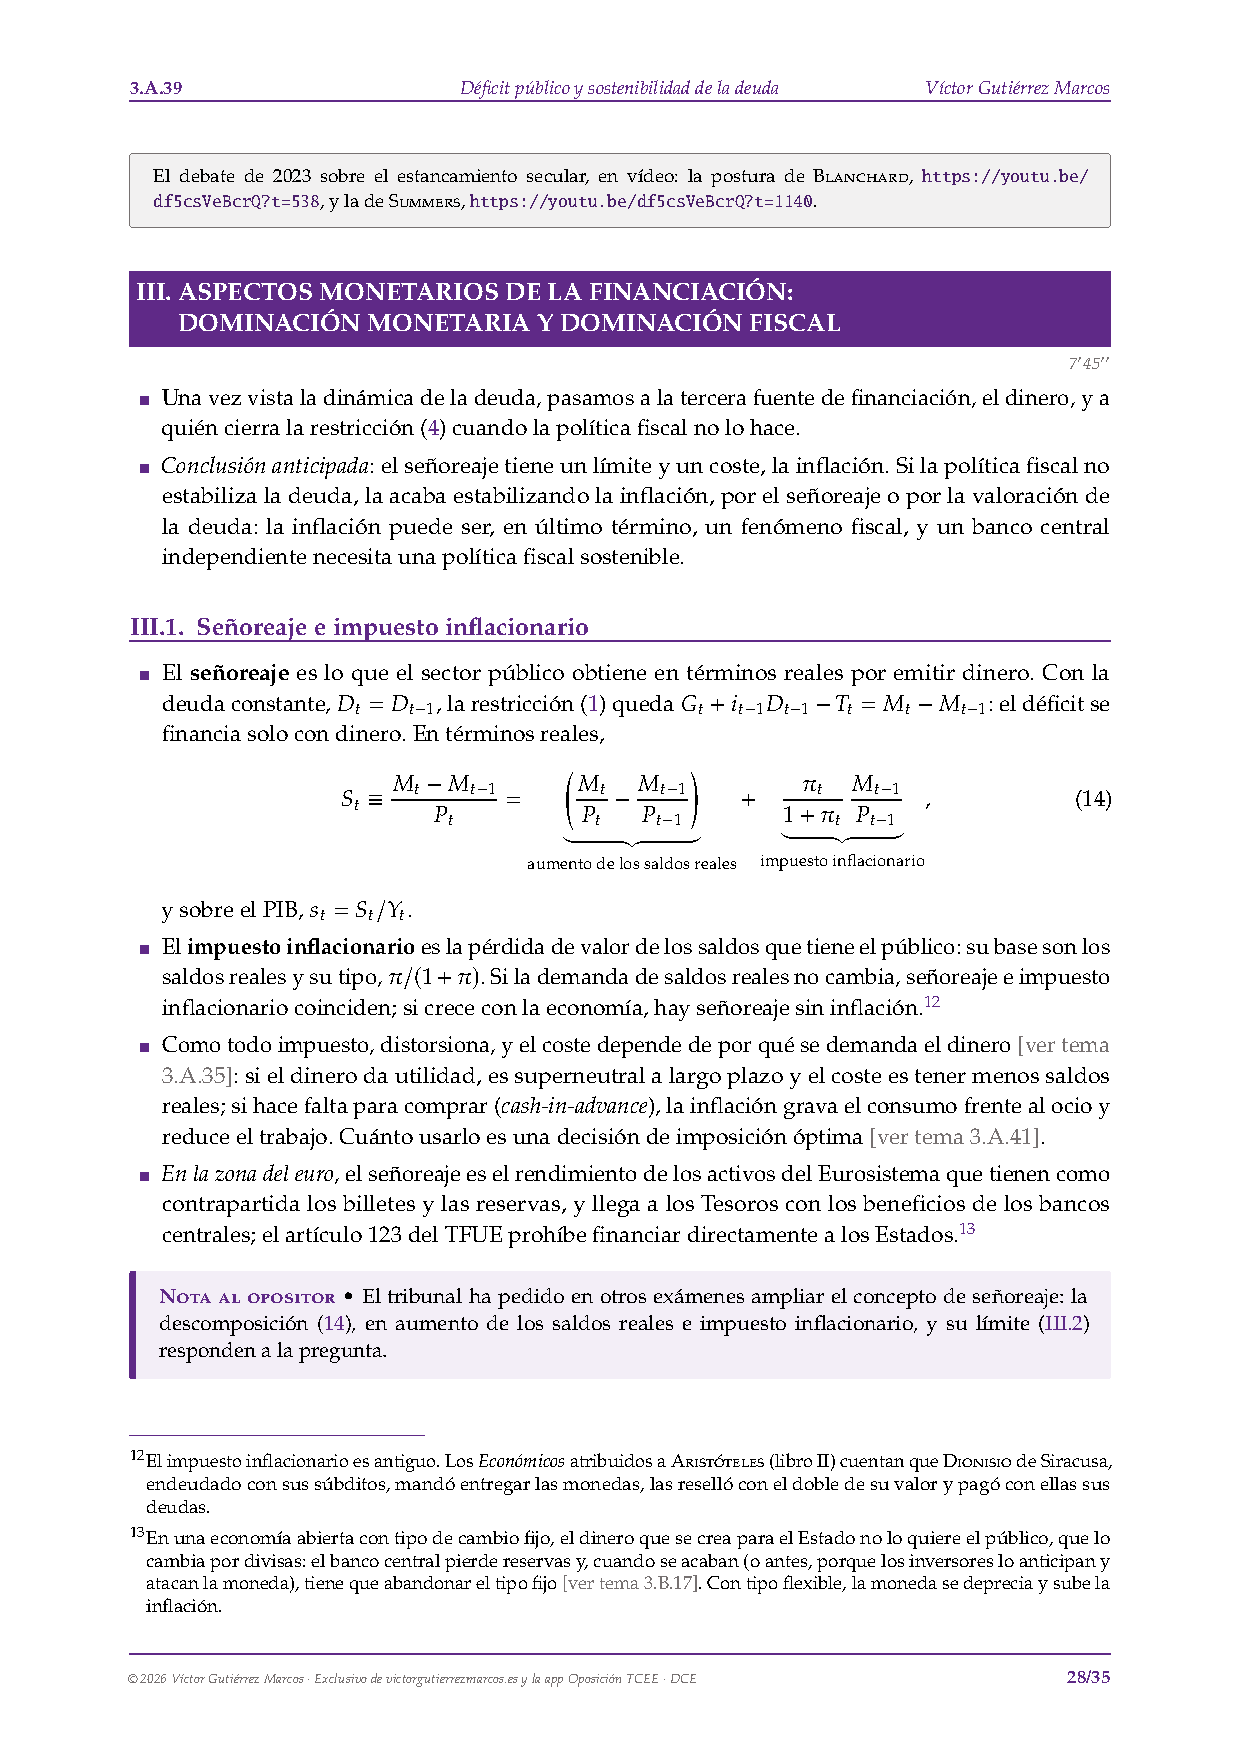
\includegraphics[width=7.6cm]{pagina-3A39.pdf}};
  \draw[tceegris!70,line width=0.4pt] (pag.south west) rectangle (pag.north east);
  \begin{scope}[shift={(pag.north west)},x=0.012767cm,y=-0.012767cm]
    \draw[tceedorado,line width=0.7pt,rounded corners=1pt] (508,164) rectangle (536,182);
    \draw[tceedorado,line width=0.7pt,rounded corners=1pt] (488,491) rectangle (537,510);
    \draw[tceedorado,line width=0.7pt] (447,479) circle (6);
    \node[num] at (44,86) {1};
    \node[num] at (44,139) {2};
    \node[num] at (556,173) {3};
    \node[num] at (44,190) {4};
    \node[num] at (44,222) {5};
    \node[num] at (44,300) {6};
    \node[num] at (44,330) {7};
    \node[num] at (556,383) {8};
    \node[num] at (556,500) {10};
    \node[num] at (44,562) {9};
    \node[num] at (44,621) {11};
    \node[num] at (44,700) {12};
  \end{scope}
\end{tikzpicture}
\end{minipage}\hfill
\begin{minipage}[t]{7.75cm}\vspace{0pt}\footnotesize\raggedright
\setlength{\parskip}{3.2pt}
{\bfseries\color{tceemorado}Fuera del hilo, antes del apartado}\par
\nm{1} \emph{Caja gris} al final del apartado anterior: vídeos y lecturas para ver. Se mira, no se canta.\par
{\bfseries\color{tceemorado}Lo que se canta}\par
\nm{2} \emph{Título del apartado} (I, II o III), en mayúsculas: responde a una pregunta de la problemática.\par
\nm{3} \emph{Minutos} del apartado, en gris a la derecha: \tiempo{7,75} de los 30.\par
\nm{4} \emph{Nexo}: la primera viñeta enlaza con el bloque anterior («Una vez vista la dinámica de la deuda, pasamos a…»).\par
\nm{5} \emph{Conclusión anticipada}, en cursiva: lo que el apartado va a demostrar, dicho antes de demostrarlo.\par
\nm{6} \emph{Subapartado}: un concepto o un modelo cada uno.\par
\nm{7} \emph{Concepto en negrita} la primera vez que sale, con su definición en la misma frase: «El \textbf{señoreaje} es lo que el sector público obtiene…».\par
\nm{8} \emph{Ecuación numerada}, con una llave bajo cada término que dice qué es: la interpretación analítica, leída en palabras. Si se queda en la pizarra todo el cante, va en morado (función clave).\par
\nm{9} \emph{Aplicación}: tras el mecanismo, el caso europeo o español, con el arranque en cursiva («\emph{En la zona del euro}, …»).\par
{\bfseries\color{tceemorado}Lo que se mira y no se canta}\par
\nm{10} \emph{Remisión} en gris, \emph{detrás} de la idea: \vertema{3.A.35}. En voz alta se dice el contenido, nunca el número.\par
\nm{11} \emph{Nota al opositor}: qué ha preguntado el tribunal en otros exámenes y cómo responderlo con lo que ya está en el tema.\par
\nm{12} \emph{Nota al pie}, con su llamada en el texto: el matiz o la curiosidad que ameniza sin cortar el hilo (aquí, que el señoreaje ya existía en tiempos de \autor{Dionisio} de Siracusa).\par
\end{minipage}
\fuente{elaboración propia a partir del 3.A.39 (página 28 de 35).}
\end{infografia}

\subsection{Un concepto, 3 interpretaciones}\label{sec:concepto}

\begin{itemize}
\item \textbf{\emph{La regla}}: cada concepto importante se da con su \emph{definición} (una frase que se dice tal cual), su \emph{interpretación analítica} (la fórmula, leída en palabras) y su \emph{interpretación gráfica} (dónde se ve en el gráfico). Con las 3, el tribunal ve que se entiende y no solo que se recuerda.
\item \textbf{\emph{En el tema}}: la definición va con el concepto en negrita; la fórmula, en una ecuación o como función clave; el gráfico, en una figura que se dibuja por capas. La derivación, si es corta, va en nota al pie (figura~\ref{figu:concepto}).
\end{itemize}

\begin{infografia}[!tb]
\centering
\caption{Un concepto en sus 3 interpretaciones: el índice de \autor{Lerner} en el 3.A.17 (monopolio)}\label{figu:concepto}
\begin{tikzpicture}[inf]
  \foreach \i/\t in {0/{1. Definición},1/{2. Interpretación analítica},2/{3. Interpretación gráfica}}
    \node[paso,text width=4.75cm,minimum height=0.8cm] (h\i) at (\i*5.3,0) {\t};
  \node[que,text width=4.75cm,minimum height=4.05cm,anchor=north] (c0) at ($(h0.south)+(0,-0.2)$)
    {El \textbf{índice de \autor{Lerner}} mide el \emph{poder de mercado} como el margen relativo del precio sobre el coste marginal.\\[5pt]
     Una frase, la misma siempre, que se dice tal cual: quita las preguntas sobre la definición, en las que es más fácil perder puntos que ganarlos.};
  \node[que,text width=4.75cm,minimum height=4.05cm,anchor=north] (c1) at ($(h1.south)+(0,-0.2)$)
    {\makebox[4.75cm]{\fcolorbox{tceemorado}{tceemoradopalido}{\color{tceemorado}$\mathcal{L}\equiv\dfrac{p^M-\mathrm{CMg}}{p^M}=\dfrac{1}{|\varepsilon|}$}}\\[7pt]
     Se lee en palabras: \emph{el margen es la inversa de la elasticidad}; cuanto menos sustitutos tiene el bien, más margen.\\[3pt]
     La derivación, de una línea, va en nota al pie.};
  \node[que,text width=4.75cm,minimum height=4.05cm,anchor=north] (c2) at ($(h2.south)+(0,-0.2)$) {};
  \begin{scope}[shift={($(c2.south west)+(0.55,0.45)$)},x=1cm,y=1cm]
    \draw[->,thick] (0,0) -- (3.9,0) node[below left=0pt and -2pt,font=\scriptsize] {$q$};
    \draw[->,thick] (0,0) -- (0,2.95) node[left,font=\scriptsize] {$p$};
    \draw[very thick,tceemorado] (0.1,2.7) -- (3.6,0.075) node[above right=-1pt and -10pt,font=\scriptsize] {$D$};
    \draw[very thick,tceeazul] (0.1,2.65) -- (2.0,0.08) node[right,font=\scriptsize] {$\mathrm{IMg}$};
    \draw[very thick,tceeverde] (0.1,0.8) -- (3.7,0.8) node[above left=0pt and 0pt,font=\scriptsize] {$\mathrm{CMg}$};
    \fill (1.45,0.8) circle (1.5pt); \fill (1.45,1.6875) circle (1.5pt);
    \draw[dashed,tceegris] (1.45,0) -- (1.45,1.6875) -- (0,1.6875);
    \node[below,font=\scriptsize] at (1.45,0) {$q^M$};
    \node[left,font=\scriptsize] at (0,1.6875) {$p^M$};
    \draw[decorate,decoration={brace,amplitude=3pt},tceedorado,thick] (1.55,1.6875) -- (1.55,0.8);
    \draw[tceedorado,thin] (1.68,1.25) -- (2.35,2.25) node[above,font=\scriptsize,text=tceedorado,align=center,inner sep=1pt] {margen $p^M-\mathrm{CMg}$};
  \end{scope}
  \foreach \i/\t in {0/{Se dice sentado, de palabra.},1/{Se escribe y se queda en la esquina de la pizarra: es función clave.},2/{Se dibuja por capas: demanda, ingreso y coste marginales, equilibrio y margen.}}
    \node[ejemplo,text width=4.75cm,anchor=north] at ($(c\i.south)+(0,-0.2)$) {\t};
\end{tikzpicture}
\fuente{elaboración propia a partir del 3.A.17 (gráfico ilustrativo, sin escala).}
\end{infografia}

\subsection{Los patrones que se repiten en el cuerpo}\label{sec:patrones-cuerpo}

\begin{itemize}
\item \textbf{\emph{Las mismas formas en los 90 temas}}: además del hilo y de los modelos a)-e), hay 6 maneras de ordenar el contenido que vuelven en todo el temario. Reconocerlas ayuda a estudiar (cada forma se memoriza igual) y a improvisar un tema que no se tiene revisado (figura~\ref{figu:patrones}).
\end{itemize}

\begin{infografia}[!tb]
\centering
\caption{Los 6 patrones que se repiten en el cuerpo de los temas}\label{figu:patrones}
\begin{tcbraster}[raster columns=2,raster equal height=rows,raster column skip=3mm,raster row skip=3mm]
\tarjeta{tceemorado}{1. Dos escuelas, una viñeta cada una}{%
\fila{Cómo}{cuando se comparan 2 enfoques, cada uno en su viñeta y sus puntos debajo, sangrados: se ve de un vistazo qué dice cada uno.}
\fila{Ejemplos}{la síntesis neoclásica y el monetarismo (3.A.5); lo \emph{normativo} (utilidad esperada) frente a lo \emph{positivo} (teoría de las perspectivas), en el 3.A.10.}}
\tarjeta{tceeazul}{2. Criterio, tipo, ventajas e inconvenientes}{%
\fila{Cómo}{las clasificaciones, en 3 niveles: el criterio en cursiva («\emph{Según cómo se calcula}»), cada tipo con su concepto en negrita y, debajo, \emph{Ventaja} e \emph{Inconveniente}.}
\fila{Ejemplos}{los aranceles \emph{ad valorem}, específicos y mixtos (3.B.7); 69 pares de ventajas e inconvenientes en el temario.}}
\tarjeta{tceeverde}{3. Desarrollo por pasos}{%
\fila{Cómo}{«Paso 1, Paso 2…», cada paso en su viñeta y lo que se hace debajo: se canta igual que se escribe en la pizarra.}
\fila{Ejemplos}{los 3 pasos del paseo aleatorio de \autor{Hall} (3.A.33); más de 200 pasos en el temario.}}
\tarjeta{tceedorado}{4. El dato, con fuente, fecha y comparación}{%
\fila{Cómo}{la última cifra oficial, primero de España y después de la UE o del mundo, con otra cifra que le da sentido; la fuente, en la bibliografía.}
\fila{Ejemplos}{el 54,4~\% de las empresas españolas no tiene asalariados y el valor añadido por ocupado de las grandes es 1,7~veces el de las micro (3.B.4).}}
\tarjeta{tceenaranja}{5. Teoría, evidencia y valoración}{%
\fila{Cómo}{cada modelo termina con lo que dicen los datos (\emph{Evidencia empírica}, unos 300 bloques) y con su \emph{Valoración}, que suele abrir el siguiente apartado.}
\fila{Ejemplos}{la contrastación del paseo aleatorio tras \autor{Hall} (3.A.33); la paradoja de \autor{Leontief} tras \autor{Heckscher}-\autor{Ohlin} (3.B.5).}}
\tarjeta{tceegris}{6. Del mecanismo al caso europeo o español}{%
\fila{Cómo}{tras explicar cómo funciona algo, una viñeta lo aplica, con el arranque en cursiva: «\emph{En la zona del euro}…», «\emph{En España}…».}
\fila{Ejemplos}{el señoreaje del Eurosistema y el artículo 123 del TFUE (3.A.39); el ejemplo conductor que vuelve en cada concepto (3.A.14).}}
\end{tcbraster}
\fuente{elaboración propia a partir de los 90 temas del tercer ejercicio.}
\end{infografia}

% ==========================================================================
\section{Cómo se cuenta un modelo}\label{sec:modelo}

\begin{itemize}
\item \textbf{\emph{La estructura}}: si un apartado es un modelo, se organiza así (en algunos no se desarrolla alguno de los bloques):
  \begin{itemize}
  \item \emph{a) Idea}: objetivo, relevancia, contexto y resultados.
  \item \emph{b) Modelo}:
    \begin{itemize}
    \item \emph{i) Supuestos};
    \item \emph{ii) Desarrollo}: analítico y gráfico;
    \item \emph{iii) Implicaciones}: resultados y propiedades; implicaciones de política económica.
    \end{itemize}
  \item \emph{c) Extensiones}: qué pasa al relajar los supuestos.
  \item \emph{d) Evidencia empírica}: cómo se ve en los datos.
  \item \emph{e) Valoración}: críticas y complementariedad con los otros desarrollos expuestos. Puede servir para conectar un apartado con el siguiente.
  \end{itemize}
\item \textbf{\emph{Una estructura rígida}}: siempre esta jerarquía y este orden. Solo se pueden saltar las extensiones o la evidencia empírica si no las hay, y entonces las letras siguen seguidas («a) Idea, b) Modelo, c) Valoración»): lo que se memoriza es el nombre del bloque, no la letra.
\item \textbf{\emph{En el cante importan los resultados}}: el modelo no se deriva como en una clase. Se dicen los supuestos que hacen falta, se escribe la ecuación clave y el gráfico, y el tiempo se guarda para las implicaciones y la valoración.
\end{itemize}

\begin{infografia}[!tb]
\centering
\caption{Un modelo de a) a e), con lo que se dice y lo que va a la pizarra: el paseo aleatorio de \autor{Hall} (1978) en el 3.A.33}\label{figu:modelo}
\begin{tikzpicture}[inf]
\matrix (m) [matrix of nodes,ampersand replacement=\&,row sep=2mm,column sep=2.5mm,
  nodes={anchor=center},
  column 1/.style={nodes={paso,text width=2.35cm}},column 2/.style={nodes={ejemplo,text width=7.4cm}},column 3/.style={nodes={pizarra}}]
{
 |[cabecera,fill=none,text width=2.35cm]| Bloque \& |[cabecera,fill=none,draw=none,font=\footnotesize\bfseries\upshape,text=tceemorado]| Lo que se dice \& |[cabecera,fill=none,draw=none]| En la pizarra \\
 a) Idea \& Con expectativas racionales, solo las noticias cambian el consumo: el mejor predictor del consumo de mañana es el de hoy. \autor{Hall} plantea el problema de \autor{Fisher} y \autor{Friedman} con renta incierta. \& |[pizarra,text=tceegris]| \emph{nada: de palabra} \\
 |[pasoclaro]| i) Supuestos \& Utilidad esperada con expectativas racionales; utilidad cuadrática; un activo sin riesgo y $\beta(1+r)=1$. \& $u(C)=C-\tfrac{b}{2}C^2$,\quad $\beta(1+r)=1$ \\
 |[pasoclaro]| ii) Desarrollo \& El problema con su restricción; la ecuación de \autor{Euler} estocástica y 3 pasos: la utilidad marginal es una martingala, es lineal y la esperanza la atraviesa, y el error de predicción tiene media cero. \& {\fcolorbox{tceemorado}{tceemoradopalido}{\color{tceemorado}$u'(C_t)=\beta(1+r)\,\mathbb{E}_t[u'(C_{t+1})]$}\\[3pt] \fcolorbox{tceemorado}{tceemoradopalido}{\color{tceemorado}$C_{t+1}=C_t+\varepsilon_{t+1}$}} \\
 |[pasoclaro]| iii) Implicaciones \& El cambio del consumo no se puede predecir; solo importan las sorpresas; lo permanente pesa más que lo transitorio; crítica de \autor{Lucas}; la IS dinámica del modelo neokeynesiano. \& |[pizarra,text=tceegris]| \emph{de palabra} \\
 c) Valoración \& La utilidad cuadrática excluye el motivo precaución; mercado de capitales perfecto. «Si los datos rechazan el paseo aleatorio, el fallo puede estar en cualquiera de esas piezas.» \& |[pizarra,text=tceegris]| {\emph{de palabra:}\\ \emph{puente a la contrastación}} \\
};
\node[draw=tceemorado,rounded corners=2pt,fit=(m-3-1)(m-5-1),inner sep=2.5pt,label={[font=\scriptsize\bfseries,text=tceemorado,rotate=90,anchor=south]left:b) Modelo}] {};
\foreach \i [evaluate=\i as \j using int(\i+1)] in {2,...,5} \draw[flechamorada] (m-\i-1) -- (m-\j-1);
\node[font=\scriptsize\itshape,text=tceegris,align=left,anchor=north west,text width=15.5cm] at ($(m.south west)+(0,-1mm)$) {Sin extensiones ni evidencia propias (la evidencia es el apartado siguiente), así que las letras siguen seguidas: a) Idea, b) Modelo, c) Valoración. Las 2 ecuaciones recuadradas son las \emph{funciones clave}: van en morado en el tema y se quedan en una esquina de la pizarra mientras se usan.};
\end{tikzpicture}
\fuente{elaboración propia a partir del 3.A.33.}
\end{infografia}

\subsection{Los patrones de los modelos en el temario}\label{sec:patrones-modelo}

\begin{itemize}
\item \textbf{\emph{Cuántos}}: 80 de los 90 temas cuentan al menos un modelo con la estructura a)-e) en el cuerpo, 437 en total (4,9 por tema; 17 en el 3.A.24). Los 10 que no tienen ninguno son institucionales o de contabilidad: la UE, la OMC y el FMI (3.B.22, 3.B.33-3.B.37, 3.B.39, 3.B.41 y 3.B.42) y la contabilidad nacional (3.A.30).
\item \textbf{\emph{Títulos propios}}: a)-e) son títulos de nivel 4 (negrita cursiva) e i)-iii) de nivel 5 (cursiva), con la letra a mano. Si en un mismo subapartado van varios modelos, el nombre de cada uno es el título y sus bloques bajan un nivel (3.A.9).
\item \textbf{\emph{Funciones clave en morado}}: 83 temas tienen al menos una (294 en total; 13 en el 3.A.33): la ecuación que el opositor escribiría y conservaría en la pizarra, recuadrada. Por ejemplo, el índice de \autor{Lerner} en el 3.A.17 o la ecuación de \autor{Euler} en el 3.A.33.
\item \textbf{\emph{Problemas de optimización con las restricciones debajo}}, cada una en su línea, para ver el objetivo por un lado y las restricciones por otro:
  \[\optim{\max}{\{C_t\}}{\mathbb{E}_0\Big[\textstyle\sum_{t=0}^{\infty}\beta^t\,u(C_t)\Big]}{b_{t+1}=(1+r)\,b_t+Y_t-C_t\\ b_0\ \text{dado}}\]
\item \textbf{\emph{Desarrollos por pasos}}: «Paso 1, Paso 2…», cada uno en su viñeta con lo que se hace debajo (los 3 pasos de \autor{Hall}).
\item \textbf{\emph{Mismo modelo, misma forma}}: un modelo que sale en varios temas se cuenta con los mismos supuestos, la misma notación y el mismo gráfico, adaptado a la pregunta de cada tema y más extenso en su tema de referencia. En 3.A.16-3.A.19 (competencia perfecta, monopolio, competencia monopolística y oligopolio) se parte de la misma lista de supuestos y se marca cuál se levanta.
\item \textbf{\emph{Gráficos por capas}}: cada gráfico se dibuja en el orden en que se haría en la pizarra (ejes, primera curva, equilibrio y proyecciones, desplazamiento, nuevo equilibrio), que es el orden del vídeo del cante.
\end{itemize}

% ==========================================================================
\section{La pizarra}\label{sec:pizarra}

\begin{itemize}
\item \textbf{\emph{Cuándo}}: no se abusa de la pizarra; se usa solo cuando hace falta y con un fin explicativo (cuanto más didáctico, mejor): gráficos, fórmulas clave y, si ayuda, el esquema. La introducción y la conclusión se cantan sin pizarra.
\item \textbf{\emph{Sentado o de pie}}:
  \begin{itemize}
  \item La introducción y la conclusión se cantan siempre \emph{sentado}. El cuerpo, sentado cuando no se va a usar la pizarra.
  \item Se canta \emph{de pie} solo para usar la pizarra (después de la introducción se puede uno levantar si quiere llamar la atención del tribunal, pero no es lo habitual).
  \end{itemize}
\item \textbf{\emph{Cómo}}: escribir grande y claro, que se vea bien; después de usarla, se borra.
\item \textbf{\emph{Entre apartados}}: se borra todo salvo las funciones clave (y algún gráfico central) a las que se volverá; se dejan en una esquina.
\end{itemize}

\begin{infografia}[!tb]
\centering
\caption{La pizarra de un apartado: qué se escribe y dónde (monopolio, 3.A.17)}\label{figu:pizarra}
\begin{tikzpicture}[inf,
  num/.style={circle,fill=tceedorado,text=white,font=\scriptsize\bfseries,inner sep=1pt,minimum size=4mm}]
  % marco de la pizarra
  \draw[line width=3pt,tceegris!70,rounded corners=3pt] (0,0) rectangle (15.6,7.2);
  \fill[white] (0.08,0.08) rectangle (15.52,7.12);
  \fill[tceegris!50,rounded corners=1pt] (4,-0.25) rectangle (11.6,-0.05);
  % columnas
  \fill[tceemoradopalido] (0.1,0.1) rectangle (3.7,7.1);
  \draw[tceegris!60,dashed] (3.7,0.2) -- (3.7,7.0);
  \draw[tceegris!60,dashed] (10.5,0.2) -- (10.5,7.0);
  \node[font=\scriptsize\bfseries,text=tceemorado,align=center] at (1.9,6.6) {ESQUINA\\ QUE SE QUEDA};
  \node[font=\scriptsize\bfseries,text=tceegris,align=center] at (7.1,6.75) {GRÁFICO, POR CAPAS};
  \node[font=\scriptsize\bfseries,text=tceegris,align=center] at (13,6.75) {PASOS Y FÓRMULAS};
  % esquina
  \node[draw=tceemorado,fill=white,line width=0.8pt,rounded corners=2pt,text=tceemorado,align=center,font=\footnotesize] at (1.9,5.3)
     {$\mathcal{L}\equiv\dfrac{p^M-\mathrm{CMg}}{p^M}=\dfrac{1}{|\varepsilon|}$};
  \node[text width=3.2cm,align=center,font=\scriptsize\itshape,text=tceemoradooscuro] at (1.9,3.95) {índice de \autor{Lerner}: se escribe en I.2 y se conserva todo el cante};
  \node[draw=tceemorado,fill=white,line width=0.8pt,rounded corners=2pt,text=tceemorado,align=center,font=\footnotesize] at (1.9,2.4)
     {$\dfrac{p_i-\mathrm{CMg}_i}{p_i}=\dfrac{1}{|\varepsilon_i|}$};
  \node[text width=3.2cm,align=center,font=\scriptsize\itshape,text=tceemoradooscuro] at (1.9,1.2) {la discriminación de precios se escribe al lado y se vuelve a la primera};
  % gráfico del monopolio
  \begin{scope}[shift={(4.45,0.8)},x=1.02cm,y=1.25cm]
    \draw[->,thick] (0,0) -- (5.2,0) node[below left=1pt and 0pt] {$q$};
    \draw[->,thick] (0,0) -- (0,4.5) node[left] {$p$};
    \node[num] at (-0.35,-0.3) {1};
    \draw[very thick,tceemorado] (0.1,3.83) -- (4.9,0.23) node[above right=0pt and -2pt] {$D$};
    \node[num] at (0.45,4.2) {2};
    \draw[very thick,tceeazul] (0.1,3.75) -- (2.45,0.22) node[right] {$\mathrm{IMg}$};
    \node[num] at (2.95,0.55) {3};
    \draw[very thick,tceeverde] (0.2,0.66) -- (4.6,1.98) node[below right=-1pt and -4pt] {$\mathrm{CMg}$};
    \node[num] at (4.3,2.25) {4};
    \fill (1.833,1.15) circle (1.6pt);
    \fill (1.833,2.525) circle (1.6pt);
    \draw[dashed,tceegris] (1.833,0) -- (1.833,2.525) -- (0,2.525);
    \node[below] at (1.833,0) {$q^M$};
    \node[left] at (0,2.525) {$p^M$};
    \node[num] at (2.25,2.85) {5};
    \fill[tceedorado,opacity=0.25] (1.833,2.525) -- (3.143,1.543) -- (1.833,1.15) -- cycle;
    \node[num] at (2.75,2.2) {6};
  \end{scope}
  % pasos
  \node[text width=4.6cm,align=left,font=\footnotesize] at (13.05,4.35) {
    $\displaystyle\max_q\ p(q)\,q-C(q)$\\[6pt]
    CPO: $\mathrm{IMg}(q^M)=\mathrm{CMg}(q^M)$\\[6pt]
    $p^M\Big(1-\dfrac{1}{|\varepsilon|}\Big)=\mathrm{CMg}$\\[6pt]
    $|\varepsilon|>1$: tramo elástico};
  \node[text width=4.6cm,align=left,font=\scriptsize\itshape,text=tceegris] at (13.05,1.4) {se borra al cambiar de apartado; la esquina se queda};
\end{tikzpicture}

\vspace{2pt}
\begin{tikzpicture}[inf]
  \node[text width=15.5cm,align=left,font=\scriptsize] {\textcolor{tceedorado}{\textbf{1-6}}: el orden en que se dibuja, que es el del texto y el del vídeo: \textbf{1} ejes y rótulos; \textbf{2} la demanda; \textbf{3} el ingreso marginal; \textbf{4} el coste marginal; \textbf{5} el equilibrio $\mathrm{IMg}=\mathrm{CMg}$ y sus proyecciones; \textbf{6} la pérdida de eficiencia. Cada capa se nombra al dibujarla: la voz no se para mientras se escribe. Solo gráficos y fórmulas: texto, casi nunca.};
\end{tikzpicture}
\fuente{elaboración propia a partir del 3.A.17 (gráfico ilustrativo, sin escala).}
\end{infografia}

\subsection{Los patrones de la pizarra en el temario}\label{sec:patrones-pizarra}

\begin{itemize}
\item \textbf{\emph{El plan de la pizarra está en el tema}}: las notas al opositor que empiezan por «En el cante» (124 en el temario) dicen, apartado por apartado, qué se dibuja, cuánto dura y qué es de profundización. En el 3.B.4: «el hilo es un árbol de 2 ramas, “tamaño óptimo: sí / no”, con los autores de cada rama»; el gráfico de las estructuras de gobierno se dibuja por capas y se conserva hasta las alianzas del bloque III.
\item \textbf{\emph{Gráficos imprescindibles y de apoyo}}: de los 8 o 9 gráficos que tiene de media un tema, solo unos pocos se dibujan; los demás (datos, 3 dimensiones, mapas) se describen de palabra y quedan en el documento para estudiar.
\item \textbf{\emph{Refranes y dichos en la pizarra}}: en los temas de conceptos, un dicho corto se dice una vez al presentar el concepto y se apunta a su lado (3.A.20: «más sabe el loco en su casa…», «el que algo quiere, algo le cuesta»).
\end{itemize}

% ==========================================================================
\section{La conclusión}\label{sec:conclusion}

\begin{itemize}
\item \textbf{\emph{Qué es}}:
  \begin{itemize}
  \item Llamamos conclusión al apartado final. Es posiblemente la parte más importante junto a la introducción, porque te asegura la atención del tribunal. Por eso no hay que reducir su contenido ni su tiempo por llegar más ajustado: si falta tiempo, se recorta dentro de un apartado, nunca la conclusión.
  \item Debe huir de zanjar un debate (si se ha planteado uno) o de extraer las lecciones del tema (eso se ha ido haciendo en cada apartado para que no se pierda quien escucha). Difícilmente el opositor resolverá oralmente en unos minutos un debate que los círculos académicos tratan por escrito.
  \item Un buen apartado final recopila lo visto, si es necesario, pero sobre todo abre el tema al resto del temario o a cuestiones no tratadas, para suscitar preguntas y asegurar a quien escucha que el opositor puede tratar otras cuestiones además de las expuestas.
  \end{itemize}
\item \textbf{\emph{Recapitulación}}: empieza por «En conclusión,». Dar las ideas clave en un breve resumen, sin que sea una mera repetición del contenido del cante.
\item \textbf{\emph{Relevancia}}: remarcar la relevancia del tema mostrando fascinación.
\item \textbf{\emph{Extensiones y relación con otras partes del temario}}: aplicaciones de lo estudiado en otros ámbitos (líneas de investigación actuales, aplicabilidad…). Es «tirar la caña» al tribunal con temas que controlemos, para provocar preguntas que sabemos responder.
\item \textbf{\emph{Opinión}}: una postura fundada y \emph{corta}, de 2 a 4 viñetas; donde encaja, con una frase célebre de un economista que la resume (figura~\ref{figu:opinion}).
\item \textbf{\emph{Idea final}} (salida o cierre): por ejemplo, la respuesta a la problemática planteada al principio. Es la última frase: nunca se termina dando las gracias ni con «y con esto termino».
\end{itemize}

\begin{infografia}[!tb]
\centering
\caption{La conclusión en 5 pasos y el cierre que vuelve al principio (3.B.4)}\label{figu:conclusion}
\begin{tikzpicture}[inf]
\matrix (m) [matrix of nodes,ampersand replacement=\&,row sep=2.2mm,column sep=2.5mm,
  nodes={anchor=center},
  column 1/.style={nodes={paso}},column 2/.style={nodes={que}},column 3/.style={nodes={ejemplo,text width=7.05cm}}]
{
 |[cabecera,fill=none,text=tceemorado,text width=2.75cm]| Paso \& |[cabecera,fill=none,draw=none]| Qué se dice \& |[cabecera,fill=none,draw=none,font=\footnotesize\bfseries\upshape,text=tceemorado]| Cómo lo hace el 3.B.4 \\
 1. Recapitulación \& «En conclusión,» y una idea por bloque, con otras palabras. \& Las empresas crecen hasta donde lo permiten la tecnología y los costes de usar el mercado, o sin tamaño de destino; la vía depende de lo específicos que sean los activos; y para decidirlo hay que valorar. \\
 2. Relevancia \& Por qué importa, con un dato distinto del de la introducción. \& El tamaño pesa en la productividad, los salarios y la competencia; en España, las empresas de 250 trabajadores o más son el 0,2~\% del total. \\
 {3. Extensiones\\[-1pt]{\scriptsize\mdseries y relación con otras partes del temario}} \& Otros enfoques y temas: la «caña» para las preguntas. \& La teoría de la empresa, la inversión y el coste del capital, la estructura financiera, la eficiencia de los mercados, las opciones reales, el control de concentraciones. \\
 4. Opinión \& Una postura fundada y corta (2-4 viñetas), con evidencia; no zanja el debate. \& Desconfiar de las sinergias que se pagan por adelantado; para que las empresas crezcan, ayuda más quitar las regulaciones por umbral de tamaño que subvencionar fusiones. \\
 |[pasodorado]| 5. Idea final \& La respuesta a la pregunta del principio, volviendo al refrán. Es la última frase. \& «Roma no se hizo en un día, y tampoco se compra de un día para otro.» Crecer compensa cuando lo que se recibe vale más de lo que se paga: «el precio es lo que se paga y el valor, lo que se recibe» (\autor{Graham}). \\
};
\foreach \i [evaluate=\i as \j using int(\i+1)] in {2,...,5} \draw[flechamorada] (m-\i-1) -- (m-\j-1);
\node[rectangle,rounded corners=2pt,draw=tceedorado,line width=0.8pt,fill=tceedorado!10,text width=15.3cm,align=left,inner sep=4pt,font=\footnotesize,anchor=north west] (vuelta) at ($(m.south west)+(0,-2.5mm)$)
  {\textbf{\color{tceedorado}Cierre en círculo}: el refrán del enganche vuelve en la idea final, ya respondido. En más de 80 de los 90 temas se repite casi a la letra y en los demás se evoca: «Las desgracias nunca vienen solas: en 2020-2022 llegaron juntas una de oferta, una de demanda y otra de fuera» (3.A.32); «Volviendo al refrán, quien juega con fuego se quema, pero una casa sin fuego se hiela» (3.A.41).};
\draw[->,thick,tceedorado] (m-6-1.west) -- ++(-0.35,0) |- ($(m-2-1.west)+(0,0)$) node[pos=0.25,left,font=\scriptsize\itshape,text=tceedorado,rotate=90,anchor=south] {vuelve al enganche};
\end{tikzpicture}
\fuente{elaboración propia a partir de los 90 temas del tercer ejercicio.}
\end{infografia}

\subsection{Los patrones de la conclusión en el temario}\label{sec:patrones-conclusion}

\begin{itemize}
\item \textbf{\emph{Mismo formato que la introducción}}: 5 rótulos, cada uno solo en su línea y con el desarrollo en viñetas debajo; la recapitulación es la excepción: «\emph{Recapitulación}: En conclusión,» y las ideas debajo.
\item \textbf{\emph{La respuesta a la problemática}}: la idea final empieza muchas veces por «A la pregunta del principio…» o «Volviendo al refrán…» (3.A.43: «si se puede crecer para siempre acumulando capital, los 3 modelos responden que no»).
\item \textbf{\emph{Extensiones con remisiones}}: la caña se lanza a temas concretos, con su remisión en el texto, para que el opositor sepa qué preguntas puede provocar y dónde está la respuesta.
\end{itemize}


\subsection{La opinión}\label{sec:opinion}

\begin{itemize}
\item \textbf{\emph{Corta}}: 2 a 4 viñetas (2,3 de media), una postura clara y razonada. Lo que repite la recapitulación o adelanta la idea final, fuera.
\item \textbf{\emph{Fundada}}: con la evidencia del tema, sin zanjar el debate; el tribunal valora el criterio, no la rotundidad.
\item \textbf{\emph{Con una frase célebre donde encaja}}: 40 temas cierran la opinión con la frase de un economista que la resume. Va traducida, entre comillas, con su autor y su año; el original, en nota al pie. Ninguna frase se usa en más de 2 temas, y solo si se ha comprobado quién la dijo (muchas están mal atribuidas).
\item \textbf{\emph{3 formas}}: una postura con su porqué, 2 visiones en viñetas sangradas cuando el tema enfrenta escuelas, o la frase célebre como última viñeta (figura~\ref{figu:opinion}).
\end{itemize}

\begin{infografia}[!tb]
\centering
\caption{La opinión de la conclusión: 3 formas, con ejemplos del temario}\label{figu:opinion}
\begin{tcbraster}[raster columns=3,raster equal height=rows,raster column skip=3mm]
\tarjeta{tceemorado}{Una postura con su porqué}{%
\fila{Cómo}{2-4 viñetas: qué piensa el opositor y en qué se apoya.}
\fila{3.B.4}{comprar empresas crea valor si lleva los activos a quien mejor los gestiona, pero «conviene desconfiar de las sinergias que se pagan por adelantado»; para que las empresas crezcan, ayuda más quitar las regulaciones que saltan al cruzar un umbral de tamaño que subvencionar las fusiones.}}
\tarjeta{tceeazul}{Dos visiones, sangradas}{%
\fila{Cómo}{una viñeta por escuela o enfoque y sus razones debajo.}
\fila{3.A.5}{«Las 2 escuelas tenían parte de razón»: \emph{la síntesis}, en que la demanda importa a corto plazo y la política puede estabilizar; \emph{el monetarismo}, en que no hay atajos permanentes contra el paro, aunque la cantidad de dinero resultó un mal objetivo.}
\fila{3.A.10}{la utilidad esperada es \emph{normativa}; la teoría de las perspectivas, \emph{positiva}: «un buen análisis necesita las 2».}}
\tarjeta{tceedorado}{La frase célebre}{%
\fila{Cómo}{la última viñeta: traducción, autor y año; el original, en nota.}
\fila{3.A.1}{\autor{Joan Robinson} (1962): un modelo con toda la diversidad de la realidad sería tan poco útil «como un mapa a escala de uno a uno».}
\fila{3.A.29}{\autor{George Box} (1979): «todos los modelos son falsos, pero algunos son útiles».}
\fila{3.A.20}{\autor{Alfred Kahn}: «la mejor combinación posible de una regulación inevitablemente imperfecta y una competencia inevitablemente imperfecta».}}
\end{tcbraster}
\fuente{elaboración propia a partir de los 90 temas del tercer ejercicio.}
\end{infografia}

% ==========================================================================
\section{Nota al pie, caja gris o anexo}\label{sec:donde}

\begin{itemize}
\item \textbf{\emph{La regla}}: el cuerpo del tema es lo que se canta, en viñetas que se entienden solas. Todo lo demás se conserva, pero fuera del hilo: en una nota al pie si es breve y cuelga de una frase, en una caja gris si se consulta mientras se lee, y en un anexo si es largo, técnico o de referencia. Nada se borra por no cantarse.
\item \textbf{\emph{Para qué sirve saberlo}}: al estudiar, el cuerpo se memoriza; las notas y las cajas se leen para entender; los anexos se repasan para el test y para las preguntas del tribunal.
\item Los anexos son ampliaciones relevantes para comprender los temas o ampliar con cosas útiles de cara a los test o a posibles preguntas del tribunal.
\end{itemize}

\begin{infografia}[!tb]
\centering
\caption{¿Dónde va cada cosa? El árbol de decisión, con lo que hay en los 90 temas}\label{figu:donde}
\begin{tikzpicture}[inf]
  \tikzset{pregunta/.append style={text width=3.7cm},resultado/.append style={text width=10.6cm}}
  \node[resultado,draw=tceemorado,fill=tceemoradopalido,anchor=north west] (r1) at (3.4,0) {\textbf{\color{tceemorado}CUERPO DEL TEMA}, en viñetas que se entienden solas.\\
    -- Si es la ecuación que se queda en la pizarra: \emph{función clave}, en morado y recuadrada (294).\\
    -- Si es un consejo para cantarlo: \emph{nota al opositor}, caja morada (165, en 49 temas).\\
    -- Si es una frase para decir tal cual: \emph{idea clave}, caja verde (30).};
  \node[resultado,draw=tceeazul,fill=tceeazul!8,anchor=north west] (r2) at ($(r1.south west)+(0,-0.35)$) {\textbf{\color{tceeazul}NOTA AL PIE} \hfill 1.959 en el cuerpo, 22 por tema\\
    -- el Premio Nobel de un autor citado, con la frase del comité (540, el 28~\%);\\
    -- una remisión a otro tema para ampliar (253);\\
    -- el original de una frase célebre citada en el texto (3.A.1, 3.A.29);\\
    -- una derivación corta, un matiz o «no confundir»: «en sentido estricto, el consumo sigue una martingala» (3.A.33);\\
    -- de dónde viene un nombre: la «enfermedad holandesa» (3.B.9);\\
    -- un enlace para ver o leer, o un gráfico pequeño con su nota (la curva de la sonrisa, 3.B.11).};
  \node[resultado,draw=tceegris,fill=tceegrisclaro!55,anchor=north west] (r3) at ($(r2.south west)+(0,-0.35)$) {\textbf{\color{tceegris!70!black}CAJA GRIS} \hfill 478 en el cuerpo, 5,3 por tema\\
    -- el mapa de la exposición tras la introducción (89 temas);\\
    -- notación y siglas del tema (35); enlaces, vídeos y lecturas (83);\\
    -- tablas de datos que no se memorizan y diagramas que no se exponen (más de 100);\\
    -- un ejemplo largo o un caso: Fisher Body y General Motors (3.A.15);\\
    -- un desarrollo «paso a paso» o una anécdota biográfica.};
  \node[resultado,draw=tceedorado,fill=tceedorado!10,anchor=north west] (r4) at ($(r3.south west)+(0,-0.35)$) {\textbf{\color{tceedorado}ANEXO} \hfill 477 en los 90 temas, 5,3 por tema\\
    -- preguntas de test y del tribunal: en los 90 temas, siempre el último;\\
    -- modelos completos que no caben o no se cantan (64 temas): en la UE, los modelos van al anexo y en el cuerpo queda la idea (3.B.42);\\
    -- derivaciones y demostraciones paso a paso (33 temas), al menos tan desarrolladas como estaban;\\
    -- normativa y referencia: el reparto de competencias de la Unión (los 10 temas de la UE), cronologías (9), «qué estudia cada tema del bloque» (7).};
  \node[pregunta] (q1) at (0,0|-r1) {¿Se dice en los 30 minutos del cante?};
  \node[pregunta] (q2) at (0,0|-r2) {¿Es una precisión breve que cuelga de una frase concreta?};
  \node[pregunta] (q3) at (0,0|-r3) {¿Ayuda a entender al leer? Se mira, no se memoriza};
  \node[pregunta,draw=tceedorado] (q4) at (0,0|-r4) {Es largo, técnico o de referencia};
  \draw[flechamorada] (q1) -- node[above,font=\scriptsize\bfseries] {Sí} (r1.west|-q1);
  \draw[flechamorada] (q2) -- node[above,font=\scriptsize\bfseries] {Sí} (r2.west|-q2);
  \draw[flechamorada] (q3) -- node[above,font=\scriptsize\bfseries] {Sí} (r3.west|-q3);
  \draw[flechamorada] (q4) -- (r4.west|-q4);
  \draw[flechamorada] (q1) -- node[left,font=\scriptsize\bfseries] {No} (q2);
  \draw[flechamorada] (q2) -- node[left,font=\scriptsize\bfseries] {No} (q3);
  \draw[flechamorada] (q3) -- node[left,font=\scriptsize\bfseries] {No} (q4);
\end{tikzpicture}
\fuente{elaboración propia a partir de los 90 temas del tercer ejercicio (20/11/2026).}
\end{infografia}

\subsection{Cuándo va a nota al pie}\label{sec:nota}

\begin{itemize}
\item \textbf{\emph{Lo que ameniza sin ser central}}: las notas dan curiosidades y material para el cante sin cortar el hilo. Las bien desarrolladas se mantienen como notas, no se integran en el texto.
\item \textbf{\emph{El Premio Nobel}}: la primera vez que sale un premiado, su Nobel va en nota con la frase del comité («\autor{Friedman} recibió el Premio Nobel de Economía en 1976 “por sus logros en el análisis del consumo…”», 3.B.4). Es el tipo de nota más frecuente.
\item \textbf{\emph{Precisiones y notación}}: lo que evita un error sin interrumpir («Aquí $\alpha$ es el grado de apertura del consumo, no la participación del capital», 3.A.32); si distingue varios conceptos, en viñetas dentro de la nota.
\item \textbf{\emph{Derivaciones de una línea}}: la del índice de \autor{Lerner}, que en el texto queda como resultado y en la nota se ve paso a paso (3.A.17).
\item \textbf{\emph{El original de una frase célebre}}: en el texto, la traducción con su autor y su año; en la nota, la frase en su lengua y la obra (\autor{Joan Robinson} en el 3.A.1, \autor{George Box} en el 3.A.29).
\item \textbf{\emph{No es una nota}}: una cita de autor y año sin texto (va en el texto, «\autor{Hall} (1978)»), ni algo que se canta.
\item \textbf{\emph{Dónde hay más y menos}}: el modelo neoclásico básico lleva 35 por tema (64 el 3.A.8) y la UE, 7 (1 en el 3.B.42 y el 3.B.45): cuanto más teoría, más matices.
\end{itemize}

\subsection{Cuándo va a caja gris}\label{sec:caja}

\begin{itemize}
\item \textbf{\emph{Lo que no se canta pero ayuda a entender}}: datos de tablas imposibles de memorizar, anécdotas biográficas, desarrollos largos y material complementario, breve y en viñetas, sin perder información.
\item \textbf{\emph{Diagramas que no se exponen}}: mapas del tema, esquemas de clasificación y cronologías ilustrativas van como figura dentro de la caja; por ejemplo, el mapa de la exposición de 89 temas o los mapas por regiones del 3.B.40.
\item \textbf{\emph{La primera línea hace de título}}: «\textbf{Notación.}», «\textbf{Mapa de la exposición.}», «\textbf{Para ver.}», «\textbf{Lo que aquí no se trata.}» (3.B.35).
\item \textbf{\emph{Comprensión antes que concisión}}: cuando un pasaje es complejo, en el cuerpo va su interpretación en palabras sencillas y el desarrollo, en la caja: «De la curva aumentada al triángulo, paso a paso (para consultar; no se canta)» (3.A.41).
\end{itemize}

\subsection{Cuándo va a anexo}\label{sec:anexo}

\begin{itemize}
\item \textbf{\emph{Lo que alarga demasiado el cuerpo}}: modelos complementarios, desarrollos empíricos o enfoques históricos pasan a un anexo, nunca desaparecen. Las derivaciones que no se cantan (agregaciones de \autor{Engel} y \autor{Cournot}, condiciones de \autor{Kuhn}-\autor{Tucker}, teorema de la envolvente) también.
\item \textbf{\emph{Temas institucionales}}: en la UE y los organismos, el cuerpo no lleva modelos de teoría económica; el modelo completo, con su a)-e), va al anexo y en el cuerpo queda la idea de palabra con su remisión (el efecto Bruselas, la condicionalidad y el reparto de la ayuda, en el anexo de 3 modelos del 3.B.42).
\item \textbf{\emph{Pensamiento económico}}: las notas del tema antiguo con interés que no caben como nota se conservan en un anexo («notas de contexto», 3.A.3 y 3.A.4).
\item \textbf{\emph{El final del documento}}: tras la conclusión, salto de página; los anexos, numerados aparte (A-1, A-2…), con el de preguntas de test siempre el último, que incluye las preguntas de otros exámenes y enlaza con el simulador de test de la web; y la bibliografía en 2 partes: las \emph{fuentes esenciales} (5 como mucho) y \emph{otras referencias}.
\end{itemize}

% ==========================================================================
\section{Los patrones por tipo de tema}\label{sec:tipos}

\begin{itemize}
\item \textbf{\emph{La misma plantilla, distinto contenido}}: todos los temas comparten la introducción, el hilo, los modelos a)-e) y la conclusión; lo que cambia de un tipo a otro es cómo arrancan, qué pesa en el cuerpo y qué se lleva a los anexos.
\item \textbf{\emph{Para qué sirve}}: si sabes de qué tipo es el tema, sabes qué esperar y cómo preparar uno que no está revisado. Las cifras de las figuras son medias por tema de cada bloque del temario.
\end{itemize}


\begin{infografia}[!tb]
\centering
\caption{Los patrones por tipo de tema (I): pensamiento, micro, macro y comercio}\label{figu:tipos-a}
\begin{tcbraster}[raster columns=2,raster equal height=rows,raster column skip=3mm,raster row skip=3mm]
\tarjeta{tceemoradooscuro}{Pensamiento económico · 3.A.1-3.A.7}{%
\fila{Arranque}{refrán y una escena histórica: la reina en la LSE en 2008 (3.A.1), la estatua de \autor{Marx} en Tréveris (3.A.2).}
\fila{Cuerpo}{la escuela según \autor{Schumpeter} (líder, seguidores y cuerpo doctrinal) y, por autor, los mismos rótulos: \emph{Contexto, método y obra}; \emph{Líneas de investigación} (con sus modelos a)-e)); \emph{Recomendaciones de política económica}; \emph{Lugar en la escuela}.}
\fila{Notas y anexos}{26 notas por tema: Nobel, biografías, fechas; anexos de notas de contexto y del modelo paso a paso (3.A.5, 3.A.6).}
\fila{Remisiones}{las que más: 92 por tema (164 en el 3.A.1), porque cada escuela vuelve en el resto del temario.}}
\tarjeta{tceemorado}{Microeconomía · 3.A.8-3.A.24}{%
\fila{Arranque}{un refrán que es la intuición del tema («Sobre gustos no hay nada escrito», 3.A.8) y un mercado concreto (el aceite, 3.A.16).}
\fila{Cuerpo}{axiomas y problema de optimización con las restricciones debajo; función clave; 5-9 modelos a)-e) por tema; gráficos por capas (16 por tema en el modelo neoclásico básico). En 3.A.16-3.A.19, la misma lista de supuestos y el que se levanta.}
\fila{Notas y anexos}{muchas notas (25-35 por tema); 6-8 anexos: \autor{Kuhn}-\autor{Tucker}, envolvente, hessiana, derivaciones, «qué estudia cada tema del bloque» (bienestar).}}
\tarjeta{tceeazul}{Macroeconomía · 3.A.25-3.A.45}{%
\fila{Arranque}{refrán y un dato de España o un episodio: el PIB cayó un 10,9~\% en 2020 (3.A.42); el BCE subió tipos el 21 de julio de 2022 (3.A.37).}
\fila{Cuerpo}{familias de modelos que se suceden (clásico → keynesiano → nueva macroeconomía clásica → neokeynesiano) y la ecuación que las une: \autor{Euler}, \autor{Phillips}, IS dinámica; más funciones clave (6-7 por tema en ciclo y demanda y oferta agregadas); gráficos de datos con el último dato.}
\fila{Anexos}{el modelo paso a paso (ciclo real, \autor{Ramsey}, \autor{Sidrauski}); optimización dinámica; contabilidad nacional con cascadas de cuentas (5,7 figuras por tema).}}
\tarjeta{tceeverde}{Comercio internacional · 3.B.5-3.B.10}{%
\fila{Arranque}{un producto español: el aceite de oliva (3.B.5), los medicamentos que España vende a Alemania y le compra (3.B.6), los aranceles de 2025 (3.B.7).}
\fila{Cuerpo}{cada modelo levanta un supuesto del anterior (\autor{Ricardo} → \autor{Heckscher}-\autor{Ohlin} → competencia imperfecta → empresas heterogéneas), siempre con evidencia; muchos gráficos (12 por tema).}
\fila{Anexos}{extensiones y álgebra de los modelos (\autor{Jones}, \autor{Leontief}), el comercio exterior de España, la guerra comercial.}}
\end{tcbraster}
\fuente{elaboración propia a partir de los 90 temas del tercer ejercicio.}
\end{infografia}

\begin{infografia}[!tb]
\centering
\caption{Los patrones por tipo de tema (II): finanzas, economía abierta, organismos e historia, y Unión Europea}\label{figu:tipos-b}
\begin{tcbraster}[raster columns=2,raster equal height=rows,raster column skip=3mm,raster row skip=3mm]
\tarjeta{tceedorado}{Empresa y finanzas · 3.B.1-3.B.4, 3.B.13, 3.B.23-3.B.27}{%
\fila{Arranque}{una operación o un dato de mercado: la OPA de BBVA sobre Sabadell (3.B.4); de cada 100 dólares en fondos a largo plazo en Estados Unidos, 52 están en fondos indexados (3.B.23).}
\fila{Cuerpo}{la fórmula de valoración (valor actual, WACC, CAPM, \autor{Black}-\autor{Scholes}) con un ejemplo numérico; muchas cajas grises (6 por tema): notación, ejemplos y ratios.}
\fila{Anexos}{rentas y perpetuidades, ratios, derivaciones, ejemplos resueltos, normativa (el régimen legal de la OPA).}}
\tarjeta{tceenaranja}{Economía abierta · 3.A.32, 3.B.11-3.B.19, 3.B.29}{%
\fila{Arranque}{la balanza o el tipo de cambio de España: el déficit exterior de 2007 (3.B.11 y 3.B.12).}
\fila{Cuerpo}{identidades contables primero (balanza de pagos, paridades) y modelos después (\autor{Mundell}-\autor{Fleming}, \autor{Dornbusch}, generaciones de crisis); funciones clave (4 por tema).}
\fila{Anexos}{cuadros del manual del FMI, el modelo «paso a paso», los regímenes uno a uno.}}
\tarjeta{tceegris}{Organismos e historia · 3.B.20-3.B.22, 3.B.30, 3.B.32-3.B.35}{%
\fila{Arranque}{una fecha: el 15 de agosto de 1971 de \autor{Nixon} (3.B.21); los 80 años del FMI (3.B.22).}
\fila{Cuerpo}{origen y cronología, funcionamiento (órganos, recursos, decisiones) y debate actual; casi sin modelos (0,6 por tema en organismos) y pocas notas (8), salvo en historia (25, con fechas y personajes).}
\fila{Anexos}{cronología, «conceptos», «el tema en el temario», el modelo que no se canta (la palanca del capital de los bancos de desarrollo, 3.B.30).}}
\tarjeta{tceemorado!70!tceeazul}{Unión Europea · 3.B.36-3.B.45}{%
\fila{Arranque}{refrán y una fecha de la Unión: el 9 de mayo de 1950 de \autor{Schuman} (3.B.36), el «cueste lo que cueste» del 26 de julio de 2012 (3.B.43), el arancel «recíproco» de 2025 (3.B.41).}
\fila{Cuerpo}{la \emph{fórmula común} de las políticas (figura~\ref{figu:ue}); sin modelos en el cuerpo, solo su idea de palabra; las menos notas (7 por tema).}
\fila{Anexos}{el mismo anexo en los 10 temas, «el reparto de competencias de la Unión» (arts. 2-6 TFUE), con la competencia del tema resaltada; los modelos completos; «conceptos».}}
\end{tcbraster}
\fuente{elaboración propia a partir de los 90 temas del tercer ejercicio.}
\end{infografia}

\subsection{La fórmula común de las políticas de la UE}\label{sec:ue}

\begin{itemize}
\item \textbf{\emph{Una plantilla para 10 temas}}: cada política de la Unión se cuenta con las mismas 5 piezas, en este orden, adaptadas al título oficial y sin tocar los títulos de primer y segundo nivel.
\item \textbf{\emph{Cuando el título manda otro orden}}, se respeta y la pieza que falta se pone donde encaje: en el 3.B.43 la evolución (el SME y los criterios) va antes que la justificación, porque el título empieza por la historia; en el 3.B.44, el origen de la unión bancaria va antes que su porqué.
\end{itemize}

\begin{infografia}[!tb]
\centering
\caption{La fórmula común de las políticas de la UE, con dónde está cada pieza en el 3.B.40 (política regional)}\label{figu:ue}
\begin{tikzpicture}[inf,
  chev/.style={signal,signal from=west,signal to=east,signal pointer angle=120,fill=tceemorado,text=white,
     font=\footnotesize\bfseries,minimum height=1.1cm,text width=2.35cm,align=center,inner sep=2pt},
  bajo/.style={rectangle,rounded corners=2pt,fill=tceemoradopalido,draw=tceemorado!35,text width=2.6cm,align=left,inner sep=3pt,font=\scriptsize,anchor=north},
  ej/.style={rectangle,rounded corners=2pt,fill=tceesalvia,draw=tceesalviaoscuro,text width=2.6cm,align=left,inner sep=3pt,font=\scriptsize\itshape,anchor=north}]
  \foreach \i/\t/\c in {0/{1. Relevancia}/100,1/{2. Justificación}/88,2/{3. Evolución}/76,3/{4. Articulación}/64,4/{5. Retos de futuro}/52}
    \node[chev,fill=tceemorado!\c] (c\i) at (\i*3.12,0) {\t};
  \node[bajo] (d0) at ($(c0.south)+(0,-0.25)$) {Peso de la política: datos de gasto, regiones, población; por qué importa a España.};
  \node[bajo] (d1) at ($(c1.south)+(0,-0.25)$) {a) teoría económica;\\ b) delimitación de competencias;\\ c) marco jurídico;\\ d) toma de decisiones.};
  \node[bajo] (d2) at ($(c2.south)+(0,-0.25)$) {De los Tratados a hoy: etapas, reformas y marcos financieros.};
  \node[bajo] (d3) at ($(c3.south)+(0,-0.25)$) {Instrumentos y su funcionamiento: fondos, gestión, condicionalidad, ejecución.};
  \node[bajo] (d4) at ($(c4.south)+(0,-0.25)$) {Lo pendiente: el próximo marco, la absorción, las propuestas en curso.};
  \node[ej] (e0) at ($(d0.south)+(0,-0.2)$) {I.1.1 Importancia (83 de las 244 regiones por debajo del 75~\%)};
  \node[ej] (e1) at ($(d1.south)+(0,-0.2)$) {I.1.2-I.1.4 (política, económica e idea del modelo de capital móvil) e I.2 (art. 174 TFUE y siguientes)};
  \node[ej] (e2) at ($(d2.south)+(0,-0.2)$) {I.3 Antecedentes: evolución histórica};
  \node[ej] (e3) at ($(d3.south)+(0,-0.2)$) {I.4 Instrumentos y I.5.1 Gestión de los fondos};
  \node[ej] (e4) at ($(d4.south)+(0,-0.2)$) {I.5.2 Retos: absorción, regiones estancadas, la propuesta 2028-2034};
  \node[font=\scriptsize\bfseries,text=tceemorado,anchor=east] at ($(d0.west)+(-0.1,0)$) {};
  \node[rectangle,rounded corners=2pt,draw=tceedorado,fill=tceedorado!10,text width=15.2cm,align=left,inner sep=4pt,font=\footnotesize,anchor=north west] at ($(e0.west|-e1.south)+(-0.05,-0.3)$)
   {\textbf{\color{tceedorado}En los anexos de los 10 temas}: «el reparto de competencias de la Unión», la misma figura (exclusivas, compartidas, de coordinación y de apoyo) con la del tema resaltada, y el modelo completo con su a)-e) (capital móvil en el 3.B.40, \autor{Gordon}-\autor{Schaefer} en el 3.B.38, justo retorno en el 3.B.37). Las políticas social y de empleo del mismo 3.B.40 (II.1 y II.2) repiten la fórmula; la convergencia (III) no es una política y no la lleva.};
\end{tikzpicture}
\fuente{elaboración propia a partir de los temas 3.B.36-3.B.45.}
\end{infografia}

% ==========================================================================
\section{El día del examen}\label{sec:formales}

\subsection{Aspectos formales}\label{sec:aspectos}

\begin{itemize}
\item \textbf{\emph{Cuestiones básicas}}:
  \begin{itemize}
  \item Al examen se va en traje.
  \item Siempre se empieza por el tema de la parte A y luego el de la parte B.
  \item Señalar los cambios de apartado (ser esquemático, organizado). Incluso beber agua entre apartados.
  \end{itemize}
\item \textbf{\emph{Entre apartado y apartado}}, personalmente me gusta hacer 3 cosas:
  \begin{enumerate}
  \item mirar el cronómetro;
  \item asegurarme de que la pizarra está borrada (salvo que quiera ligar conceptos entre apartados y me sea útil alguna gráfica o función);
  \item beber agua.
  \end{enumerate}
\item \textbf{\emph{Lenguaje formal y técnico}}:
  \begin{itemize}
  \item Evitar palabras como «tema» (sustituir por «exposición»).
  \item Evitar las muletillas («vale», «¿no?», «o sea», «digamos», «bueno»).
  \item Usar conectores que guían al tribunal: «en primer lugar», «a continuación», «como acabamos de ver», «esto nos lleva a…», «recapitulando…».
  \end{itemize}
\item \textbf{\emph{Comunicar bien}}: hay que centrarse en 3 aspectos:
  \begin{itemize}
  \item \emph{postura}: posición de las manos (no gesticular en exceso), pies rectos y apoyados, no desviar la vista, tronco recto desde abajo;
  \item \emph{respiración}: para marcar las pausas;
  \item \emph{entonación}: volumen, pronunciación, cambios de entonación, remarcar lo importante (que no suene monótono).
  \end{itemize}
\item Recomiendo esta clase de \autor{Patrick Winston} en el MIT: \href{https://youtu.be/Unzc731iCUY}{\emph{How to speak}}. Como todo en la vida, comunicar bien es cuestión de tenacidad, trabajo y talento.
\end{itemize}

\subsection{Lo que más valora el tribunal}\label{sec:valora}

\begin{itemize}
\item Hay 3 cosas fundamentales y muy valoradas por los tribunales:
  \begin{enumerate}
  \item \emph{Presentación y forma de hablar en público}: ser claro al hablar en público, dividir bien el tema, que el tribunal te siga bien.
  \item \emph{Comprensión del tema}: que no sea meramente memorístico. Es importante comprender qué hay detrás de los conceptos y, por tanto, explicar las cosas con tus propias palabras para mostrar al tribunal que entiendes lo que estás cantando. También es importante ser solvente en las preguntas del tribunal.
  \item \emph{Contenido}: es importante diferenciarse del resto de los opositores buscando contenido y elaborando los temas. No quiere decir esto que los temas deban estar sacados al 100~\% de manuales.
  \end{enumerate}
\item En el diálogo posterior se responde a lo que se pregunta, con calma y por partes: definición, intuición y, si ayuda, la fórmula o el gráfico. Lo que se apuntó en las extensiones de la conclusión es lo más probable que pregunten.
\end{itemize}

% ==========================================================================
\section{Errores frecuentes}\label{sec:errores}

\begin{itemize}
\item \textbf{\emph{En la introducción}}:
  \begin{itemize}
  \item Saludar («Señores miembros del tribunal…») en lugar de leer el título y entrar en el enganche.
  \item Una introducción sin problemática o sin estructura anunciada, o una estructura que no se justifica.
  \item Gastar 5 minutos en la contextualización y tener que correr en el tercer apartado.
  \end{itemize}
\item \textbf{\emph{En el cuerpo}}:
  \begin{itemize}
  \item Empezar un apartado sin decir cuál es ni adónde va, o cerrarlo sin recapitular: el tribunal pierde el hilo.
  \item Explicar un modelo como en una clase, con toda la derivación, y quedarse sin tiempo para las implicaciones y la valoración.
  \item Mezclar los bloques del modelo (supuestos dentro del desarrollo, valoración antes de las implicaciones) o saltarse la idea.
  \item Dar un resultado sin su supuesto («la demanda tiene pendiente negativa» sin decir cuándo no) o un concepto solo por su definición, sin su expresión analítica ni su gráfico.
  \item Confundir el signo de un efecto, el orden de una desigualdad o una fecha clave.
  \item Cantar otro tema: desarrollar un modelo que pertenece a otro tema del programa en lugar de remitir a él por su contenido.
  \item Decir números de tema en voz alta («como veremos en el 3.A.9»).
  \item Dar datos aproximados y sin fecha: pocos, exactos, con fecha y fuente.
  \end{itemize}
\item \textbf{\emph{Con la pizarra}}:
  \begin{itemize}
  \item Escribir texto en lugar de gráficos y fórmulas; escribir pequeño; no borrar entre apartados o borrar la función clave a la que se va a volver.
  \item Dibujar el gráfico entero en silencio y explicarlo después: cada capa se nombra al dibujarla.
  \item Cantar la introducción o la conclusión de pie, junto a la pizarra.
  \end{itemize}
\item \textbf{\emph{Con lo que no se canta}}:
  \begin{itemize}
  \item Leer en voz alta las notas al pie o el contenido de las cajas grises: son para entender, no para cantar.
  \item Estudiar los anexos antes que el cuerpo: primero lo que se canta, luego lo que se pregunta.
  \item Dejar fuera una parte del título oficial (el tribunal lo tiene delante).
  \end{itemize}
\item \textbf{\emph{En la conclusión}}:
  \begin{itemize}
  \item Repetir el índice en lugar de recapitular las ideas; intentar zanjar un debate que la literatura no ha cerrado; no abrir el tema al resto del temario.
  \item Recortarla por ir justo de tiempo, avisar del tiempo («termino ya», «me queda poco», «para no extenderme») o terminar dando las gracias. La idea final es la última frase.
  \end{itemize}
\item \textbf{\emph{Con el tiempo}}: cortarse a los 24 minutos o pasarse a los 34. Los 30 minutos se ensayan con cronómetro: el reparto previsto se cumple.
\end{itemize}

\vspace{1.5em}
\begin{flushright}
\itshape Víctor Gutiérrez Marcos
\end{flushright}

\end{document}
